\section{Results}
\label{sec:results}
To test the filters' ability to increase general robustness of a high-order solver, we have implemented their formulation in \gls{hf} for triangular elements and performed simulations where the solver would become unstable otherwise.

We wanted to test the increase of robustness in extreme cases of grid coarseness, high Reynolds number, very low \gls{ma}, and moderate \gls{ma}. It is important to keep in mind that in these cases we are not seeking very accurate results, but rather robustness under all conditions. In order to popularize high-order methods, we need to make them as robust as their low-order counterparts while retaining their benefit of higher accuracy with less computational and setup effort.

The goal is to have a cheap stabilization strategy that preserves boundary conditions for cases in which the mesh is not necessarily perfectly appropriate for resolving the flow physics over the entire domain. This scenario arises frequently in industrial applications, where the mesh would be properly refined at regions of interest and coarse in regions that the engineer/scientist has decided are not as important for the problem at hand.

All the simulations that follow were performed using \gls{hf}\cite{lopez2014verification}. 2-D \gls{ns} equations are being solved, with varying values of \gls{ma}, \gls{re}, time-step ($\Delta t$), and filtering frequency. The common parameters are:
\begin{enumerate}[1.]
\item Four-stage, five-step, low-storage Runge-Kutta time-stepping method (\gls{rk45}) \cite{carpenter1994fourth} was used in the \gls{gpu}s, and forward Euler was used when running a simulation in CPUs
\item Polynomial solution representation ($p$) of order $4$. Rusanov Flux as a Riemann solver, and a \gls{ldg}~\cite{cockburn1998local} viscous flux.
\item Filters with width $h = 10$ and weghting parameter $\alpha = 0.8$.
\item Starting from uniform flow
\item Characteristic boundary conditions at the inflow and outflow. No-slip, isothermal wall boundary conditions at the cylinder's surface.
\item All quantities non-dimensionalized with free-stream temperature and cylinder wall temperature of $300$, reference length of $1$.
\item Flow properties: $\gamma = 1.4$, Prandtl number $\mathrm{Pr} = 0.72$, gas constant $R = 286.9 \frac{J}{Kg K}$, viscosity determined by Sutherland's law with reference temperature of $291.15 K$ and reference viscosity of $\mu = 1.827\mathrm{e}-5$
\end{enumerate}

Results of interest are shown in Table \ref{table:results}. Accuracy of the results is not expected. Nevertheless, as a reference, for the flow around a cylinder at \gls{re}$= 1e6$, $\bar{C_D} \approx 0.6$ in~\cite{achenbach1968distribution}, $\bar{C_D} \approx 0.4$ in \cite{roshko1961experiments} and $\St \approx  0.4$ in \cite{roshko1961experiments}. It is important to note that at a high \gls{re}, flow over a cylinder can result in a range of $\bar{C_D}$ and $\St$ values, as the results become highly sensitive to surface roughness and the level of free-stream turbulence~\cite{zdravkovich1997flow}. The experimental values of $\bar{C_D}$ vary from 0.17 to 0.40, and those of $\St$ from 0.18 to 0.50.

Because of the results obtained in Case 4, it is good to keep in mind that for flow around a cylinder at \gls{re}$\approx 2e2$, $\bar{C_D} \approx 1.18$ in \cite{roshko1961experiments} and $\St \approx  0.2$ in \cite{roshko1961experiments}. 


\begin{table}
%\begin{adjustwidth}{-2.1cm}{}
%    \centering
    \cellspacebottomlimit=5pt
    \cellspacetoplimit=5pt
%      \begin{center}                % keep track of old \tabcolsep
        \setlength{\oldtabcolsep}{\tabcolsep}     % 6.0pt
        \setlength{\tabcolsep}{0pt}               % so coloring doesn't run off
                                                  % ends of the table
        \renewcommand{\arraystretch}{2}         % because math expressions
                                                  % almost run into each other

\def \spacing {0.4cm}
\hspace{-2.5cm}
\begin{tabular}{c <{\hspace{\len}}c <{\hspace{\spacing}} 
c <{\hspace{\spacing}}
c<{\hspace{\spacing}} c<{\hspace{\spacing}} c<{\hspace{\spacing}} c<{\hspace{\spacing}} c<{\hspace{\spacing}} c <{\hspace{\spacing}} c <{\hspace{\spacing}} c}
          \toprule
Case & $\Ma$  & $\Delta t$ & $n_F$ & $\bar{C_D}$  &  $\mathrm{St}$ & \specialcell[b]{Flow time \vspace{-0.2cm}\\(s)} & Time steps  & \specialcell[b]{Wall time \vspace{-0.2cm}\\(hours)}& \specialcell[b]{Computing \vspace{-0.2cm}\\ Resources}\\
          \specialrule{\lightrulewidth}{0pt}{0pt} % so row-coloring aligns

1 & $0.2$ &  $5e-5$ &$1000$ &$0.9256$ & $0.1600$ & $1.2069$ &$1,675,700$ & $12.65$&  1 4-core i7 CPU \\
2 & $0.077$ & $5e-5$ &$1000$ & $0.9314$ & $0.1627$ & $15.44$ & $8,252,500$ & $11.78$ & 1 \gls{gpu}\\
3 & $0.87$ & $5e-5$ &$100$ & $1.8383$ & $0^*$ & $1.3833$ & $8,355,256$ & $12.63$ & 1 \gls{gpu}\\
4 & $0.0077$ & $1.25e-5$ &$1000$ & $ 1.18$ & $0.20$ & $53.44$ & $11,428,000$ & $59.51$ & 2 \gls{gpu}s\\

          \bottomrule
        \end{tabular}

      \caption{Summary of simulation results. All cases were run at $\Re = 1e6$ with polynomial representation of order $4$. Cases 1-3 were run using the mesh shown in Figure \ref{fig:meshes}. Case 4 was run using the mesh shown in Figure \ref{fig:meshes2}. Cases with $0^*$ Strouhal number reached an artificial steady-state.}
      \label{table:results}
%      \end{adjustwidth}
    \end{table}


\subsection{Stabilization Strategy}
In the simulations presented here, the solution inside every element in the entire domain is being filtered using Equation \ref{eqn:filter_form} every $n_F$ time-steps, where $n_F$ is an integer to be determined. No sensor is being used to detect problems in the flow.

The frequency of filter application is being chosen in the following heuristic way:
\begin{enumerate}[1.]
\item \label{item:start}Start the simulation with a specific time step and no filtering. Record at what time-step the simulation ends prematurely (produces NaN values) and note the value of the residuals at the last valid time-step.  This step usually takes no more than 1 minute.
\item \label{item:halve_dt}To ensure the simulation is ending prematurely because of grid resolution problems or presence of sharp gradients, and not because of an unstable time step, halve the time step and run the simulation again.
\item \label{item:check_res} Wait for the simulation to exit prematurely. If the residual at this last exit is close in value to the previous exiting residual, the time step in Step \ref{item:halve_dt} was stable. Set the new time step to the time step in \ref{item:halve_dt}. Otherwise, record the exiting residual and go back to Step \ref{item:halve_dt}.
\item Now that a stable time step has been found, apply the filter to the simulation every $n_F$ time steps, where $n_F$ is about $90\%$ of the number of imte-steps it took the simulation to become unstable when unfiltered.
\end{enumerate}

It would certainly be desirable to filter the solution at elements where a problem is detected. Nevertheless, this heuristic approach has so far enabled the stabilization of every case tried and de-couples the effectiveness of the filters from possible shortcomings of aliasing/shock sensors.

\subsection{Coarse mesh used in simulations}
In these tests, we have used the very coarse triangular mesh with $714$ elements shown in Figure \ref{fig:meshes}. The boundary layer is purposefully not resolved properly, as we would like to induce aliasing errors in the unfiltered calculation.

\begin{figure*}
\hspace{-1cm}
\subfloat[Full mesh view \label{fig:mesh}]{%
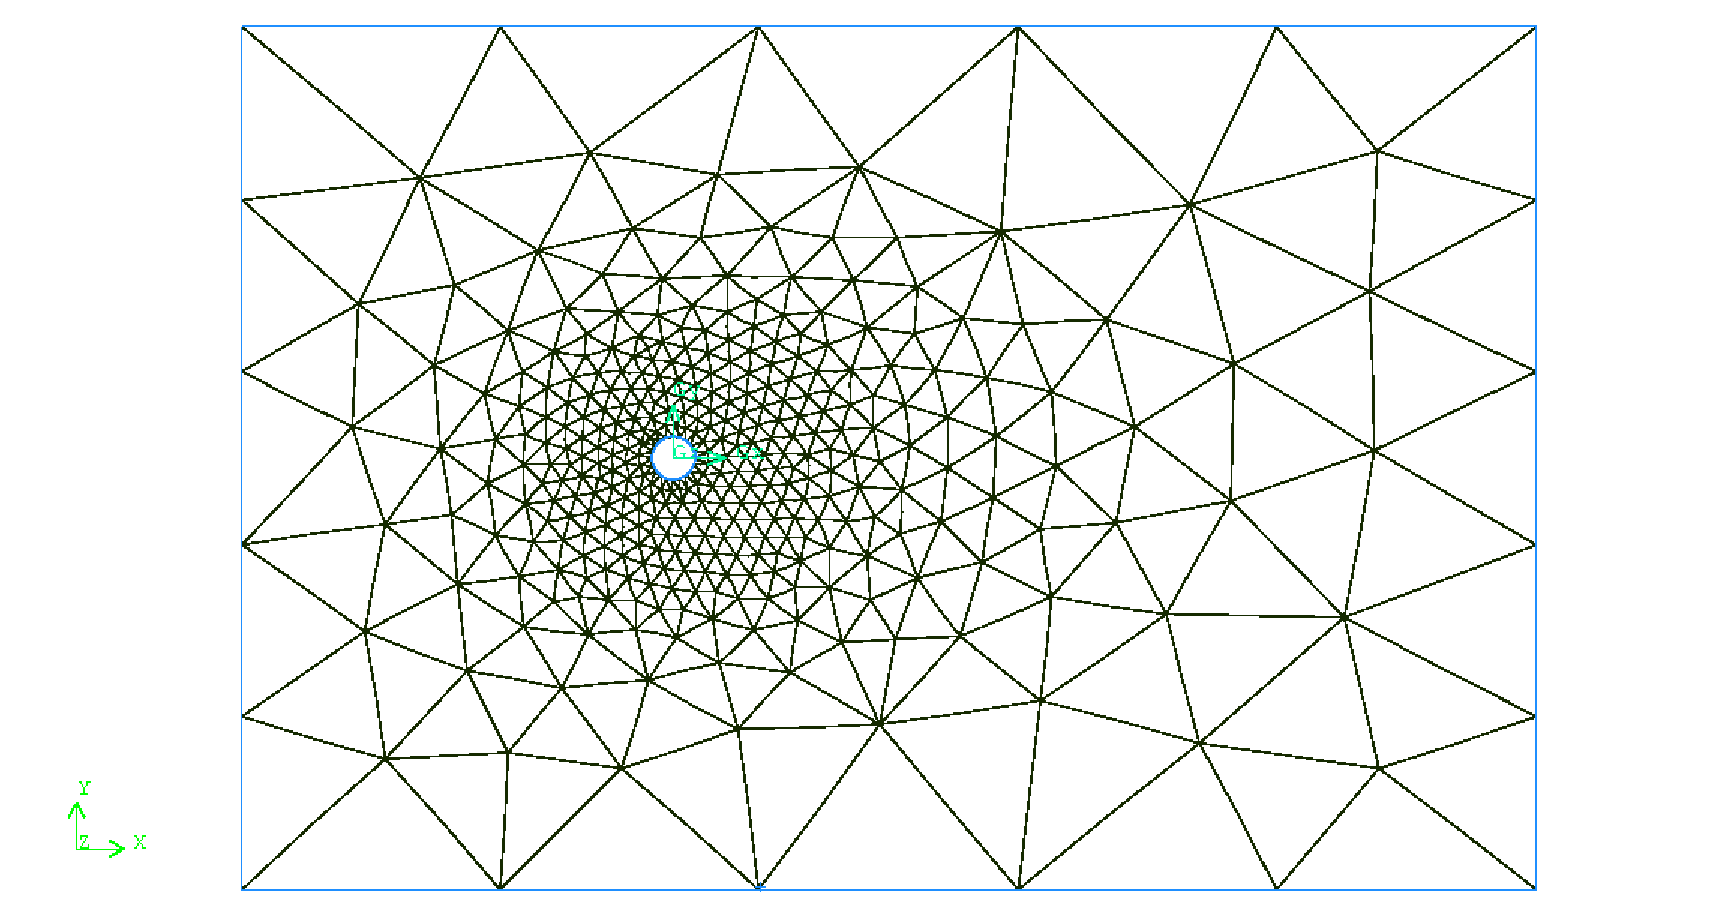
\includegraphics[width=0.55\textwidth]{\lfsdir/figs/MESH2.eps}
}
\hfill
\subfloat[Close-up view \label{fig:mesh_close}]{%
\centering
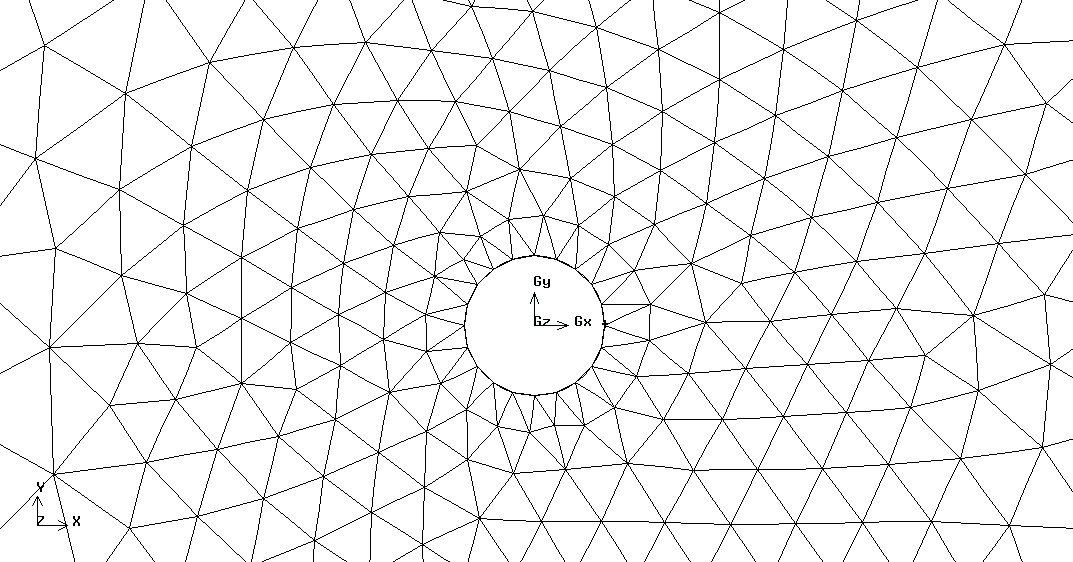
\includegraphics[width=0.55\textwidth]{\lfsdir/figs/MESH_CLOSE.png}
}
\caption{Unstructured, coarse mesh of a circular cylinder with $714$ triangular elements. Elements adjacent to the cylinder have quadratic edges.}
\label{fig:meshes}

\end{figure*}

\subsection{Flow Around a Circular Cylinder, $\bf Re =  10^6, Ma = 0.2$}
This was the first simulation performed after implementing the filters in \gls{hf}, so the \gls{gpu} implementation was not available then. The time-stepping scheme used here is simply forward Euler.

Figure \ref{fig:Ma0.2Re1e6_Ma} shows ``pretty pictures" resulting from the simulation. A video of this simulation is linked \href{https://youtu.be/b6kx8-jrK6Q}{here}.

It is interesting to note that there is a very dissipative form of vortex shedding occurring. The wake region is long, as in lower \gls{re}-number cases.

The simulation remained stable throughout and no human intervention was performed while it was occurring, from the start in uniform flow to the moment it was stopped.

From this experiment, it is unclear what portion of the numerical dissipation arises from the coarse discretization and what portion is due to the filtering operation.

This case demonstrates that the stabilization strategy can work well in cases where the mesh is improperly refined: they stabilize the solution and preserve the boundary conditions.

\begin{figure*}
\hspace{-1cm}
\subfloat[Full view \label{fig:Ma0_2Re1e6_Ma_far}]{%
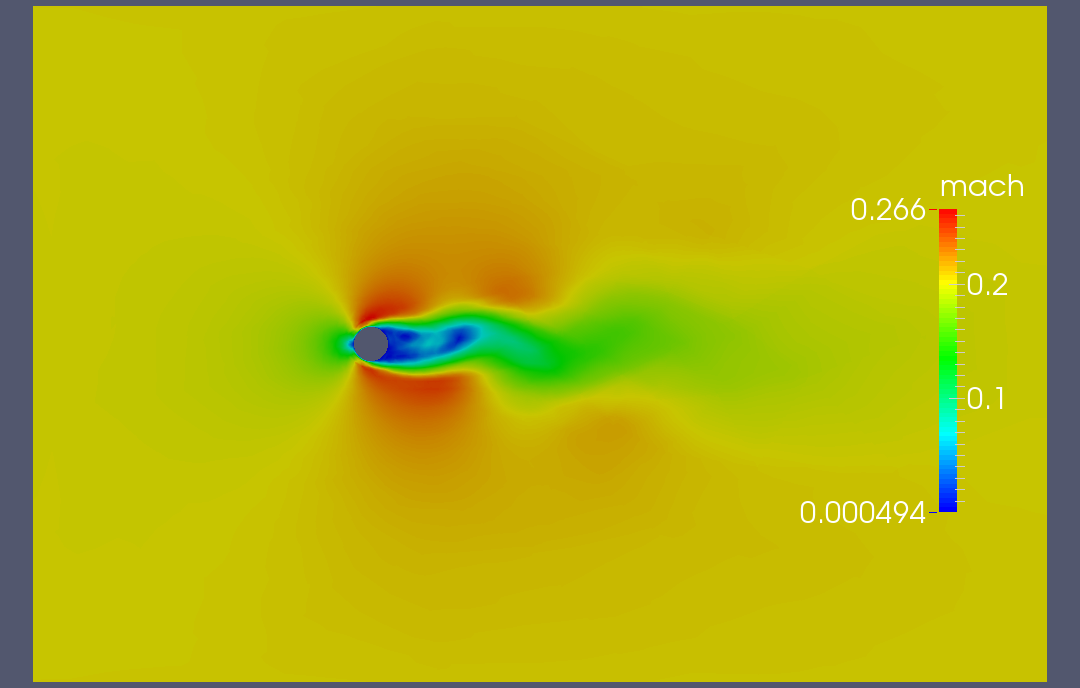
\includegraphics[width=0.55\textwidth]{\lfsdir/figs/Ma0_2--Re1e6_Ma.png}
}
\hfill
\subfloat[Close-up view \label{fig:Ma0_2Re1e6_Ma_close}]{%
\centering
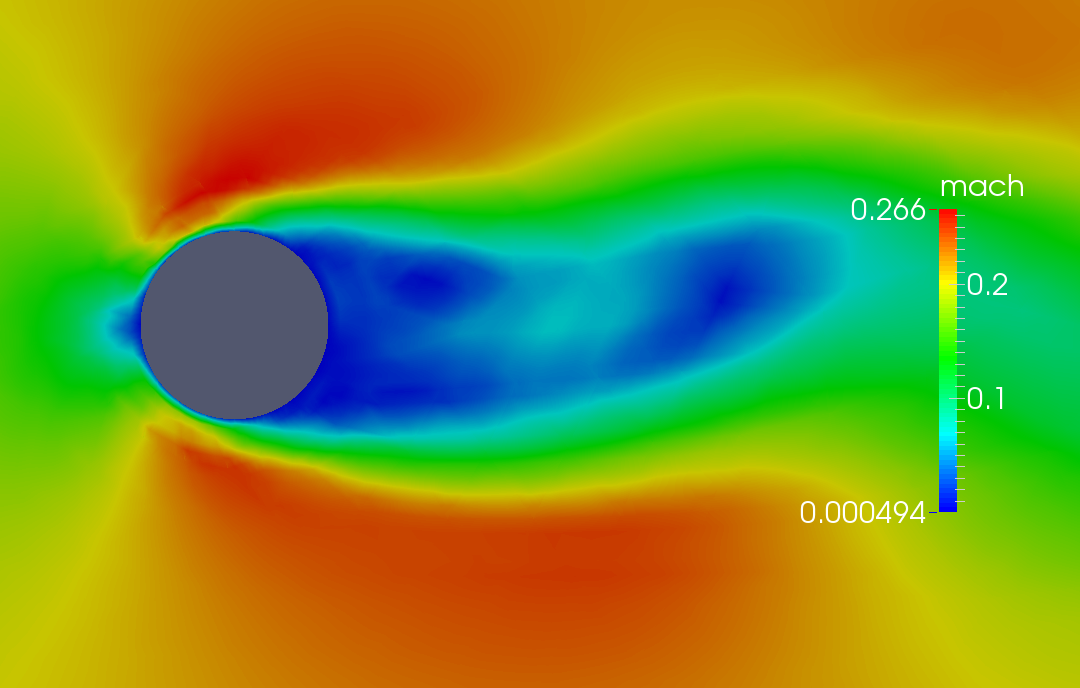
\includegraphics[width=0.55\textwidth]{\lfsdir/figs/Ma0_2--Re1e6_Ma_closeup.png}
}
\caption{Flow past a cylinder. $\Re = 1e6, \Ma = 0.2, p = 4$}
\label{fig:Ma0.2Re1e6_Ma}

\end{figure*}

\subsection{High Reynolds Number, Flow Around a Circular Cylinder, $\bf Re = 10^6, Ma = 0.077$}
This was the first simulation performed using \gls{gpu}s. The lower \gls{ma} case was of interest, as \gls{hf} had not been able to run full simulations of flows with \gls{ma}$< 0.2$.

Figure \ref{fig:Ma0.077Re1e6_Ma} shows the colorful results for this case. Once again, the boundary conditions are satisfied and the simulation is stabilized without further intervention. The same time-step size was used as in the previous case in order to leave as many parameters as possible unchanged.

A video of this simulation is linked \href{https://youtu.be/EymTVFzyPcA}{here} in real-time, and \href{https://youtu.be/8ZH349_GRUA}{here} at 0.1$\times$. A feature of these simulations that can only be appreciated by watching the linked videos is that the filters have a visible effect on the regions where aliasing and instabilities are expected: the rear part of the cylinder and the boundary layer. However, even though the filters are being applied everywhere, smooth, well-resolved regions of the flow look unchanged. To what extent the smooth regions remain unchanged has not been quantified.

\begin{figure*}
\hspace{-1cm}
\subfloat[Full view \label{fig:Ma0_077Re1e6_Ma_far}]{%
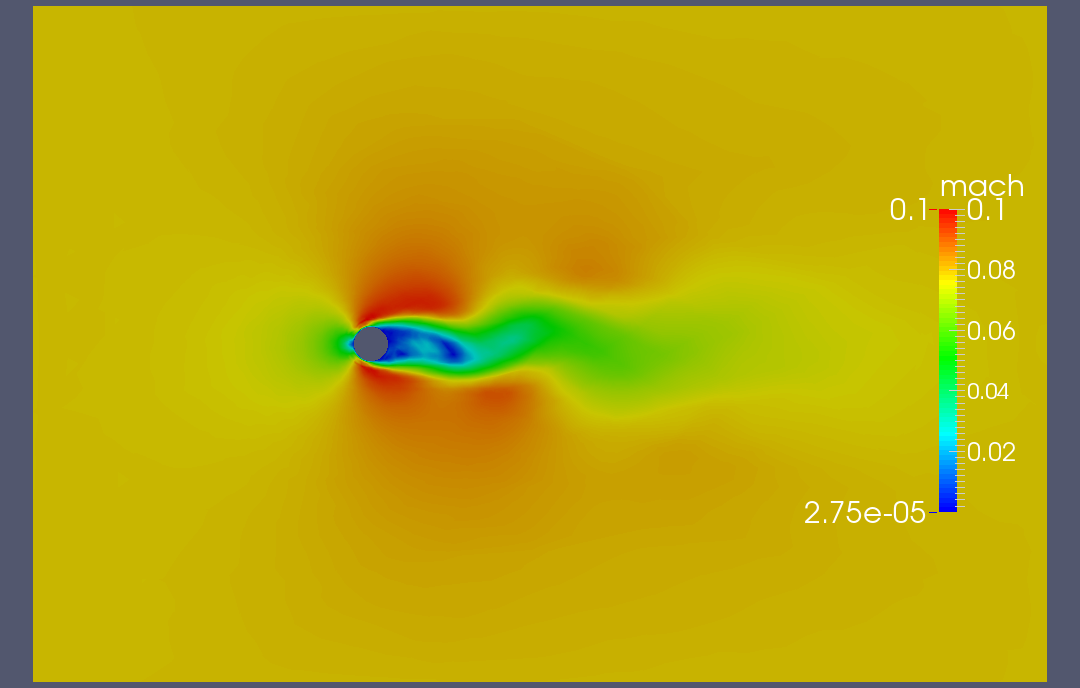
\includegraphics[width=0.55\textwidth]{\lfsdir/figs/Ma0_077--Re1e6_Ma.png}
}
\hfill
\subfloat[Close-up view \label{fig:Ma0_077Re1e6_Ma_close}]{%
\centering
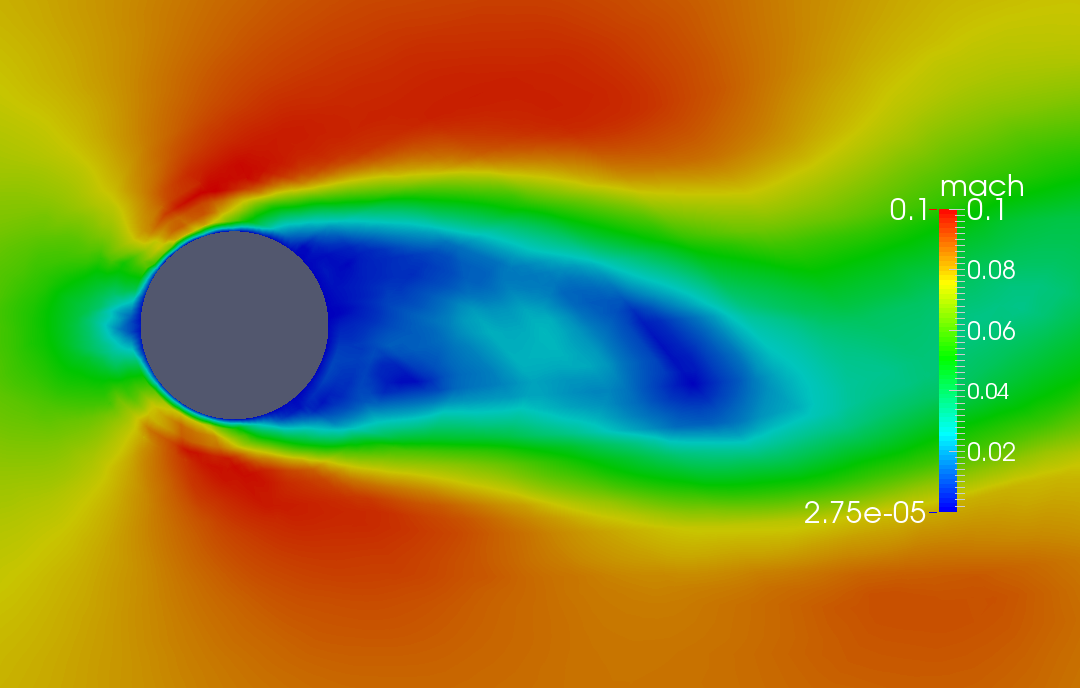
\includegraphics[width=0.55\textwidth]{\lfsdir/figs/Ma0_077--Re1e6_Ma_closeup.png}
}
\caption{Flow past a cylinder. \gls{re}$= 1e6$, \gls{ma} $= 0.077, p = 4$}
\label{fig:Ma0.077Re1e6_Ma}

\end{figure*}

%\subsection{High Reynolds Number, Flow Around a Circular Cylinder, $\bf Re = 10^6, Ma = 0.85$}

\begin{figure*}
\hspace{-1cm}
\subfloat[Full view \label{fig:Ma0_87Re1e6_Ma_unstable_far}]{%
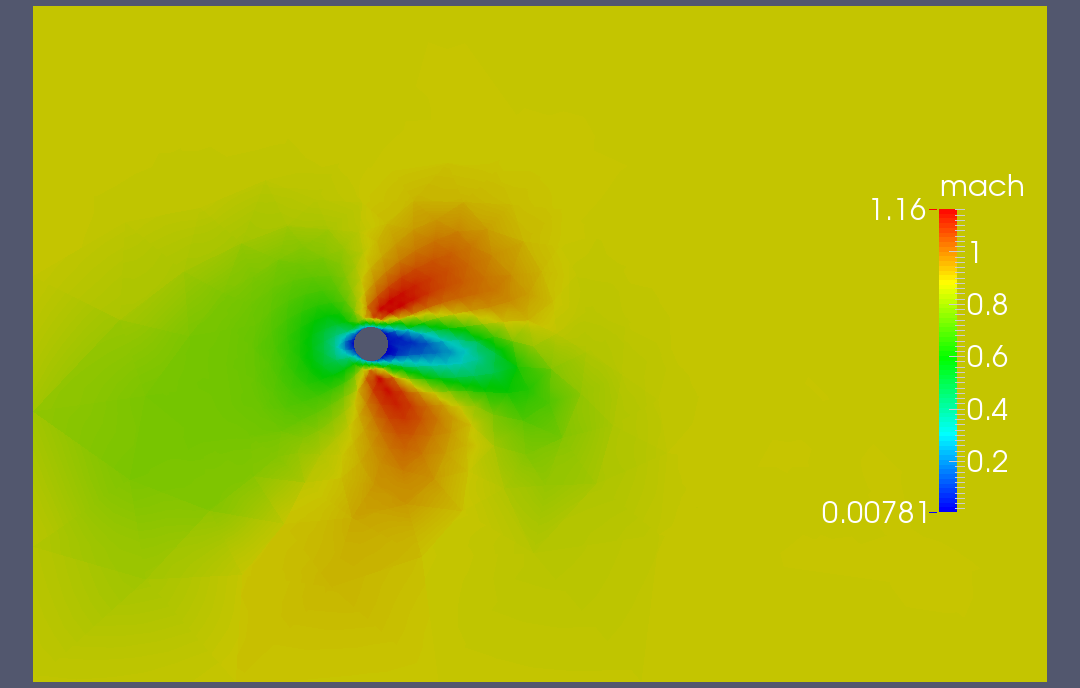
\includegraphics[width=0.55\textwidth]{figs/Ma0_87--Re1e6_Ma.png}
}
\hfill
\subfloat[Close-up view \label{fig:Ma0_87Re1e6_Ma__unstable_close}]{%
\centering
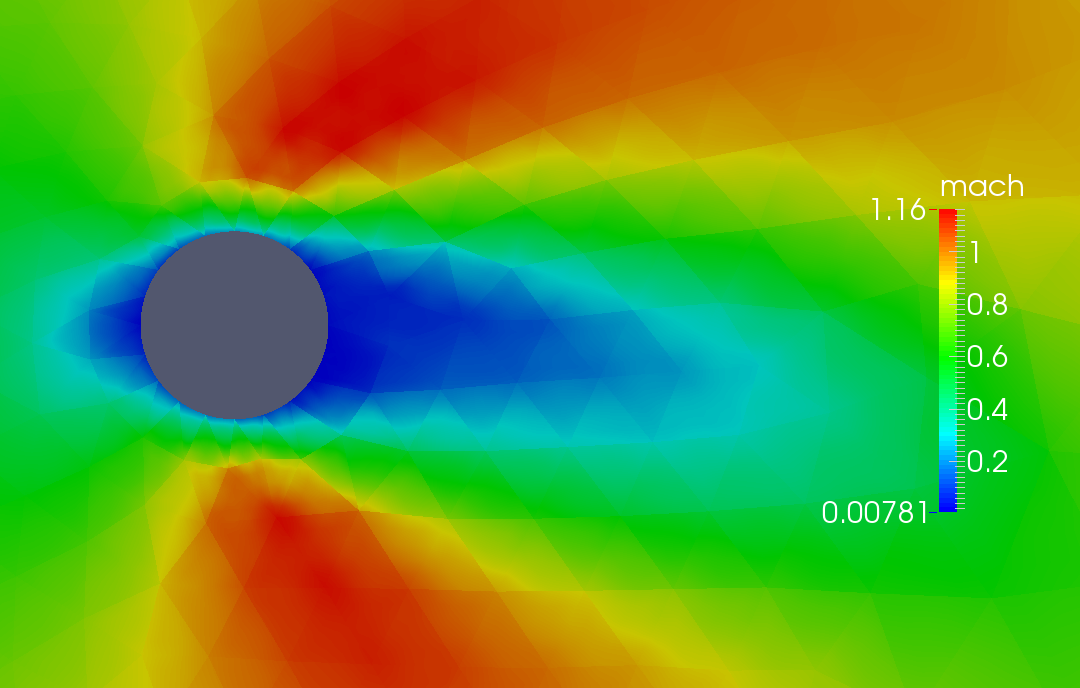
\includegraphics[width=0.55\textwidth]{figs/Ma0_87--Re1e6_Ma_closeup.png}
}

\hspace{-1cm}
\subfloat[Close-up view \label{fig:Ma0_87Re1e6_P__unstable}]{%
\centering
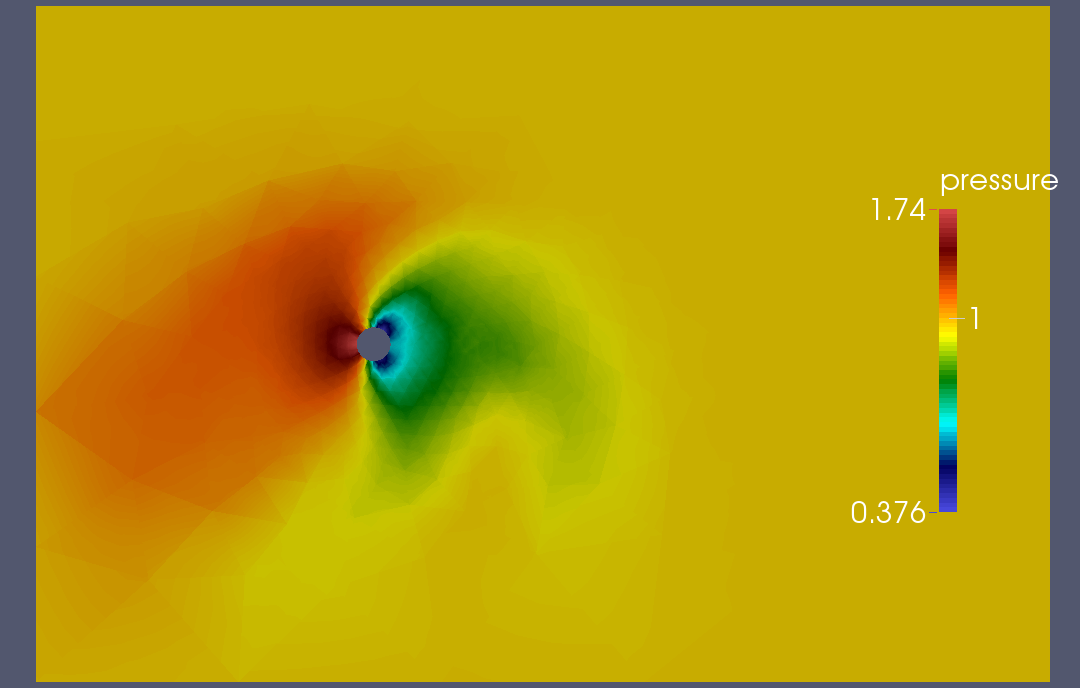
\includegraphics[width=0.55\textwidth]{figs/Ma0_87--Re1e6_P.png}
}
\hfill
\subfloat[Close-up view \label{fig:Ma0_87Re1e6_P__unstable_close}]{%
\centering
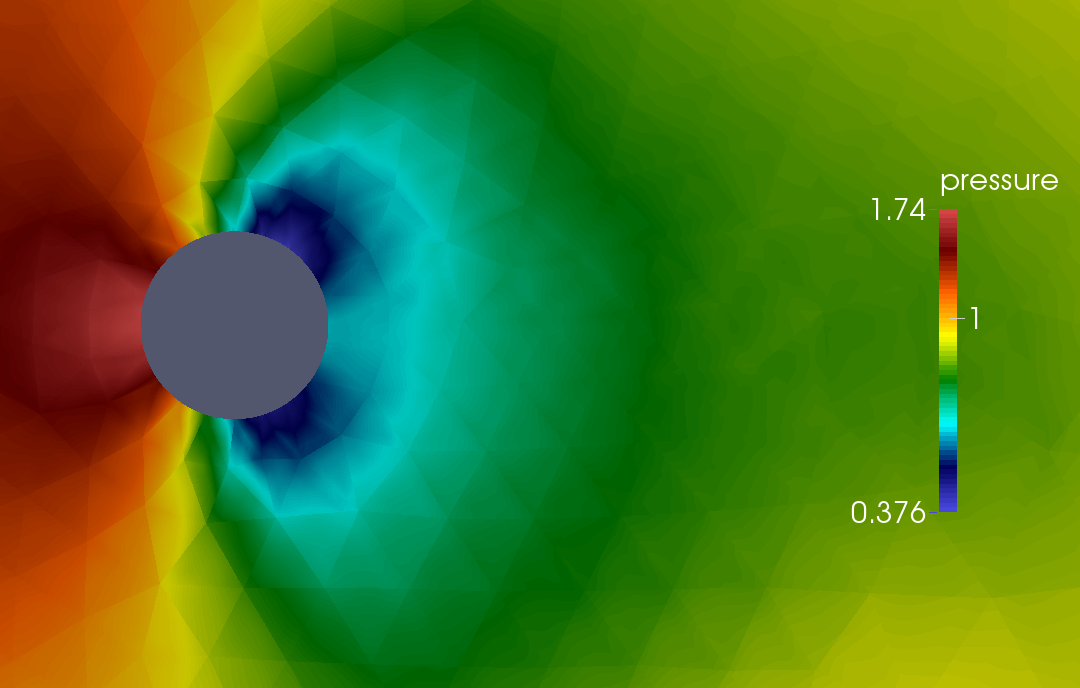
\includegraphics[width=0.55\textwidth]{figs/Ma0_87--Re1e6_P_closeup.png}
}
\caption{$\Re = 1e6, \Ma = 0.87, p = 4$}
\label{fig:Ma0.87Re1e6_unstable_Ma}
\end{figure*}

\subsection{High Reynolds Number, Flow Around a Circular Cylinder, $\bf Re = 10^6, Ma = 0.87$}

This case encompases all potential sources of instabilities in a high-order solver: poor resolution, aliasing, and sharp gradients. Figure \ref{fig:Ma0.87Re1e6} shows plots of the solution. The simulation shows a clear un-physical asymmetry due to the coarseness of the mesh. Nevertheless, the no-slip boundary conditions are being satisfied and the shock is present. 

Because of the coarseness of the mesh and the high-gradients present in the solution, quite a lot of filtering had to occur. This forced the flow to a ``steady state" and shown in the Residual and $C_D$ plots in Figure \ref{fig:Ma0.87Re1e6_history}.

\begin{figure*}
\hspace{-1cm}
\subfloat[Full view \label{fig:Ma0_87Re1e6_Ma_far}]{%
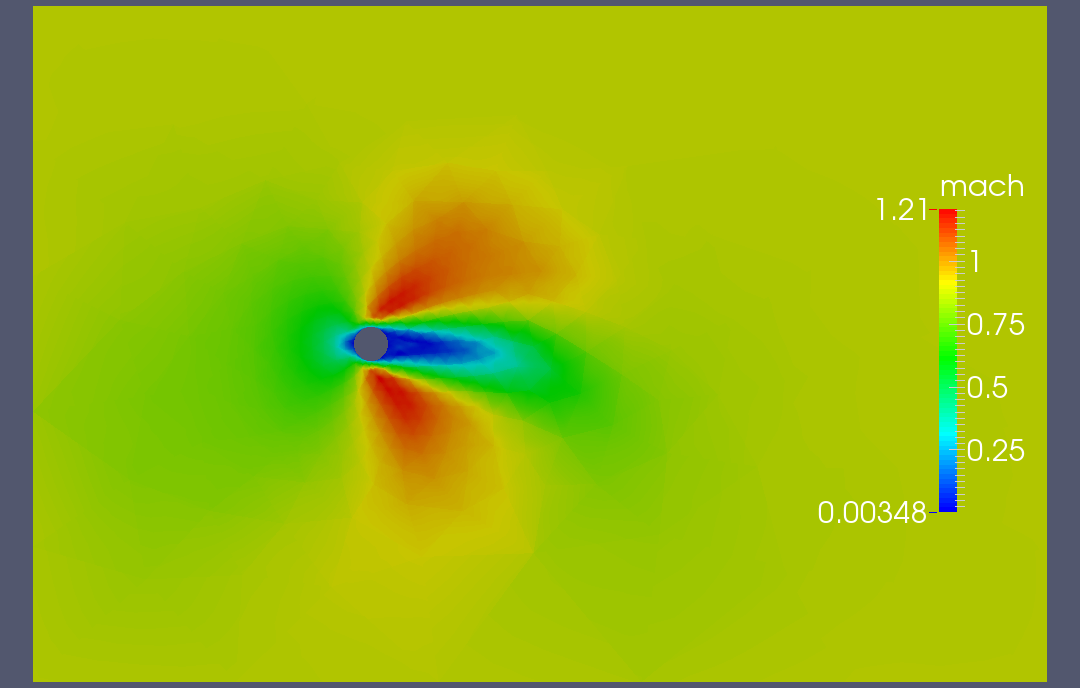
\includegraphics[width=0.55\textwidth]{\lfsdir/figs/Ma0_87--Re1e6_Ma_stable.png}
}
\hfill
\subfloat[Close-up view \label{fig:Ma0_87Re1e6_Ma_close}]{%
\centering
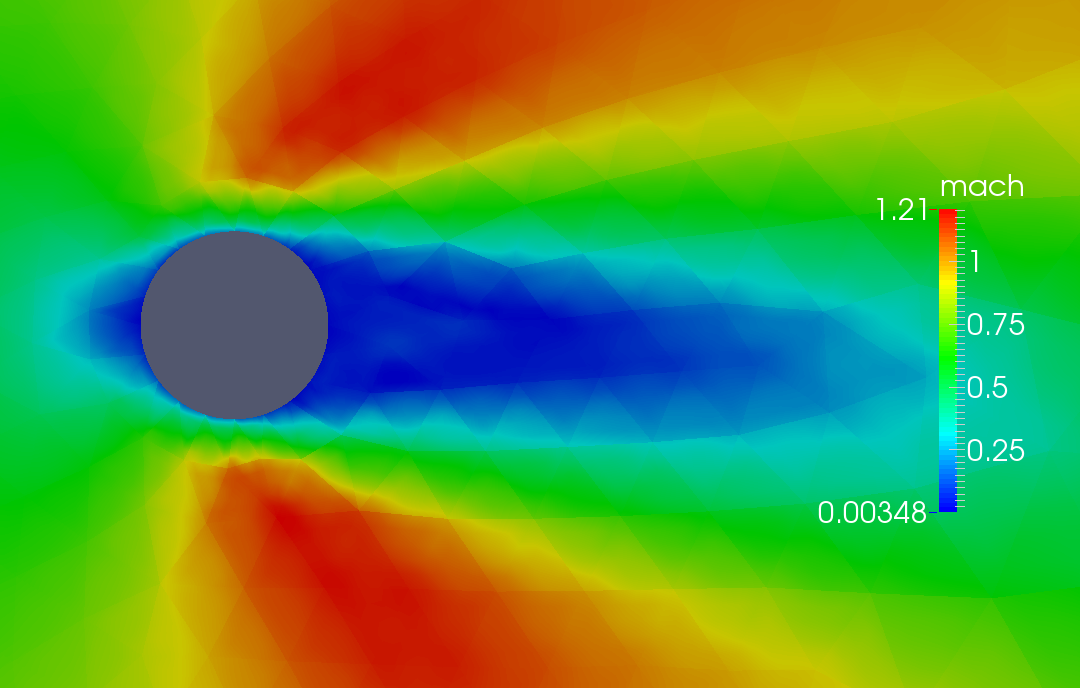
\includegraphics[width=0.55\textwidth]{\lfsdir/figs/Ma0_87--Re1e6_Ma_stable_closeup.png}
}

\hspace{-1cm}
\subfloat[Full view \label{fig:Ma0_87Re1e6_P_stable}]{%
\centering
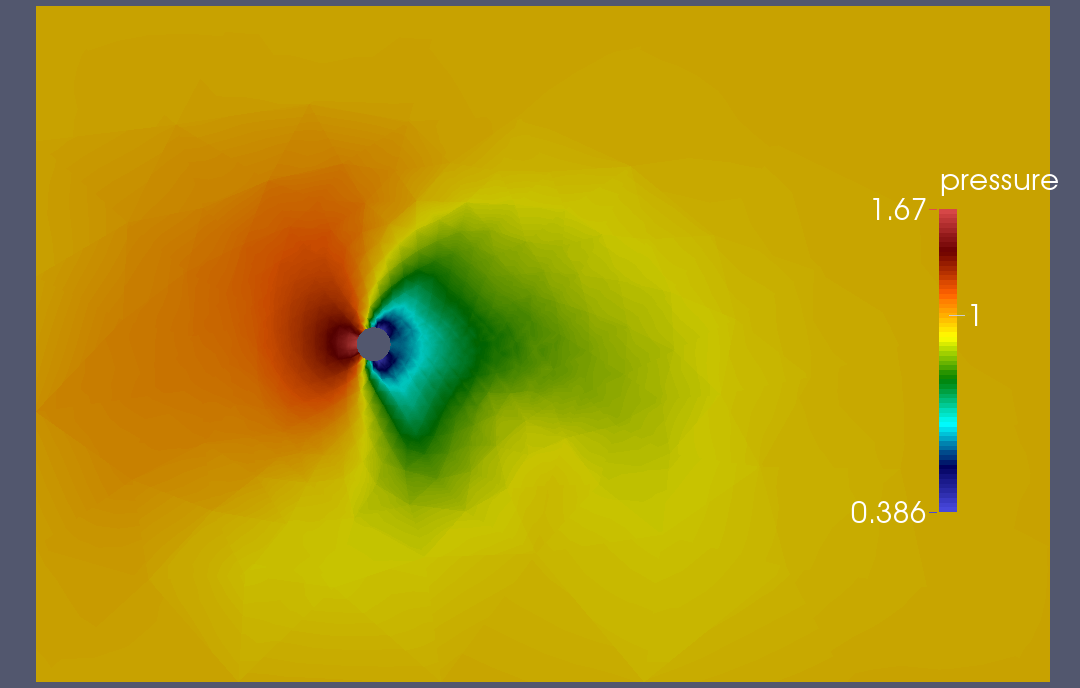
\includegraphics[width=0.55\textwidth]{\lfsdir/figs/Ma0_87--Re1e6_P_stable.png}
}
\hfill
\subfloat[Close-up view \label{fig:Ma0_87Re1e6_P_stable_close}]{%
\centering
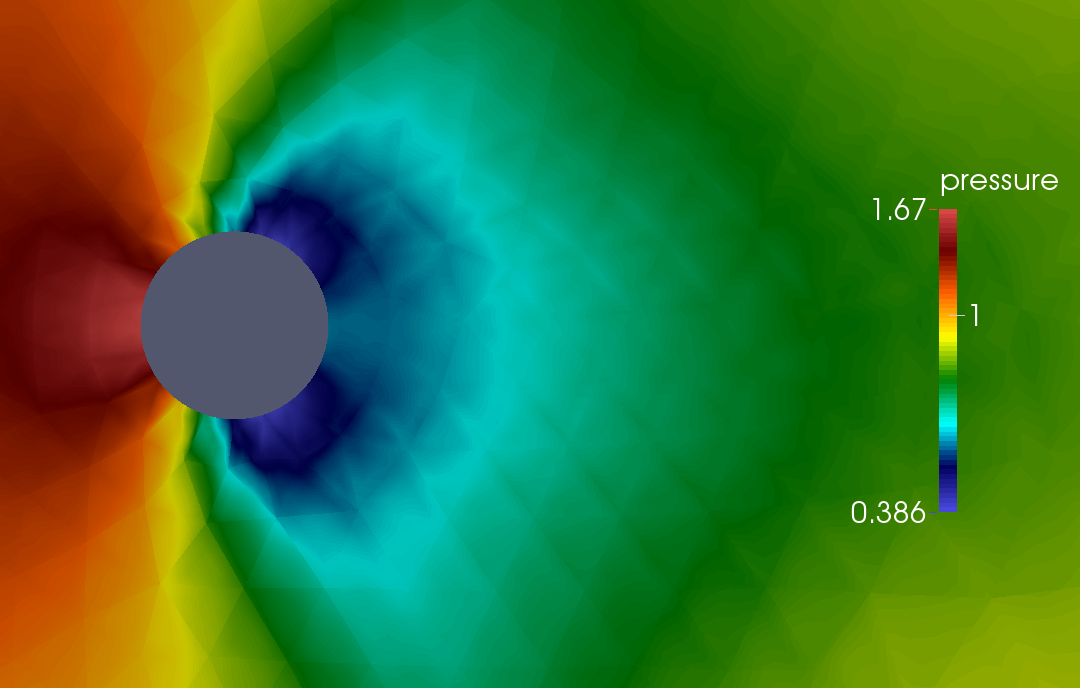
\includegraphics[width=0.55\textwidth]{\lfsdir/figs/Ma0_87--Re1e6_P_stable_closeup.png}
}
\caption{Flow past a cylinder. \gls{re}$= 1e6$, \gls{ma} $= 0.87, p = 4$}
\label{fig:Ma0.87Re1e6}

\end{figure*}

Values of $C_D$ and residual history are shown in Figure \ref{fig:Ma0.87Re1e6_history}. The value of drag ``converges" after time-step $1.846e6$. The residual in the energy conservation equation also ``converges" to a zig-zag pattern after this iteration. Figure \ref{fig:rhoE_res_history} shows the energy residual in the last few thousand time-steps. The sharp decrease in residual magnitude reveals the time-steps at which the filter is being applied.

\begin{figure*}
\subfloat[Drag coefficient history over entire simulation run. ``Steady state" is reached at time-step $1.846e6$. \label{fig:cd_history}]{%
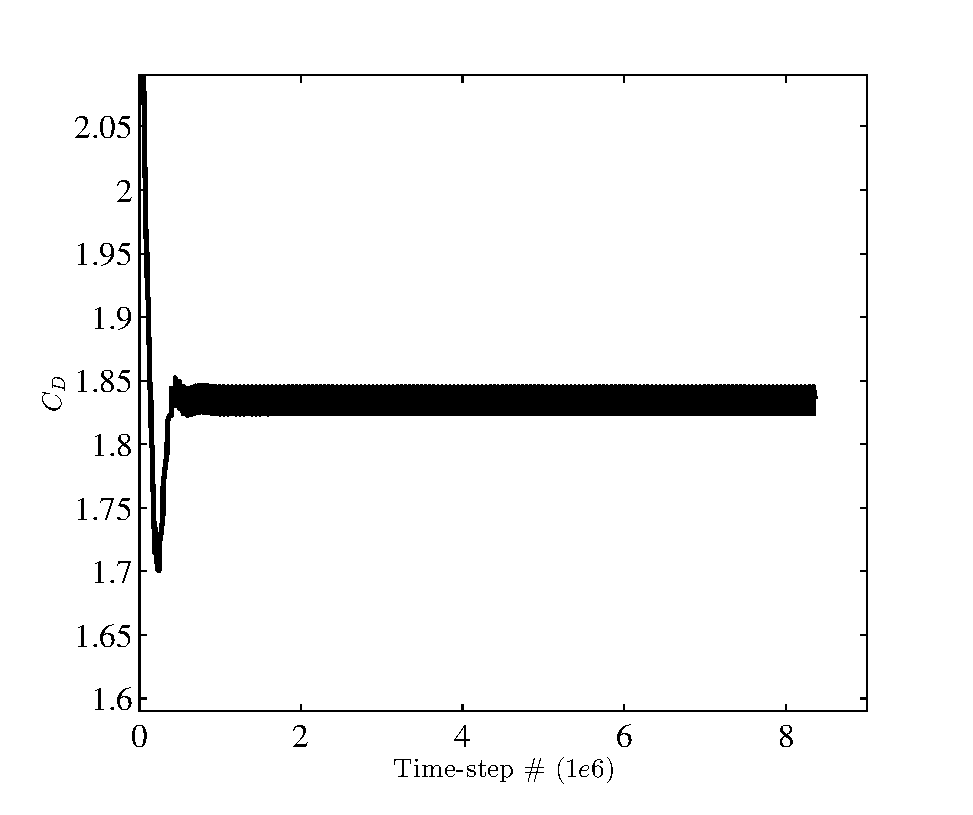
\includegraphics[width=0.55\textwidth]{\lfsdir/figs/unstable_c_d.eps}
}
\hfill
\subfloat[Energy residual history over the last few thousand time-steps \label{fig:rhoE_res_history}]{%
\centering
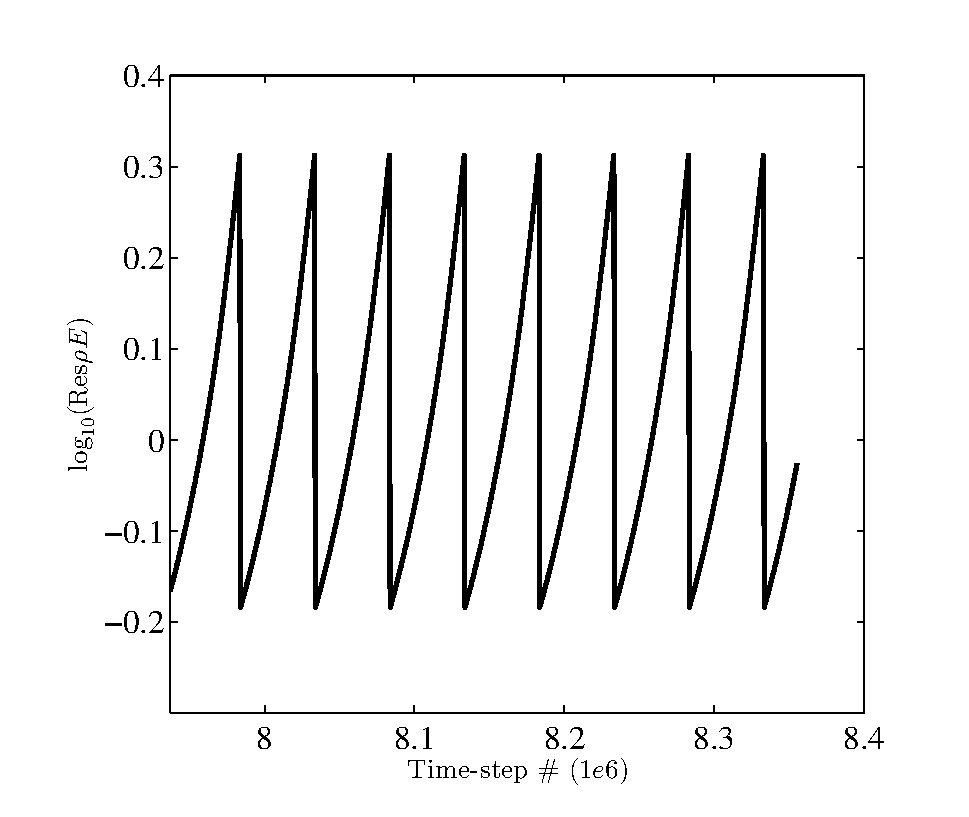
\includegraphics[width=0.55\textwidth]{\lfsdir/figs/unstable_rhoE_res.eps}
}
\caption{History of $C_D$ and energy residual of simulation in Figure \ref{fig:Ma0.87Re1e6}}
\label{fig:Ma0.87Re1e6_history}

\end{figure*}

\subsection{High Reynolds Number, Flow Around a Circular Cylinder, $\bf Re = 10^6, Ma = 0.0077$, less-coarse mesh}
This case was run with the more refined mesh seen in Figure \ref{fig:meshes2}. This mesh is still coarse for standard turbulent computations. It is interesting to note that the predicted $C_D = 1.18$ and $\mathrm{St} = 0.20$ match experimental results for \gls{re}$= 2e2$. This phenomenon could imply that the grid of the stabilized simulation determines the effective Reynolds number being simulated.

A real-time video of this simulation is linked \href{https://youtu.be/XSzWPn2fZ90}{here} for Mach contours, and \href{https://youtu.be/_zIbZgHjepY}{here} for vorticity strength contours. The filters stabilized this almost-incompressible simulation without a problem.


\begin{figure*}
\hspace{-1cm}
\subfloat[Full mesh view \label{fig:mesh2}]{%
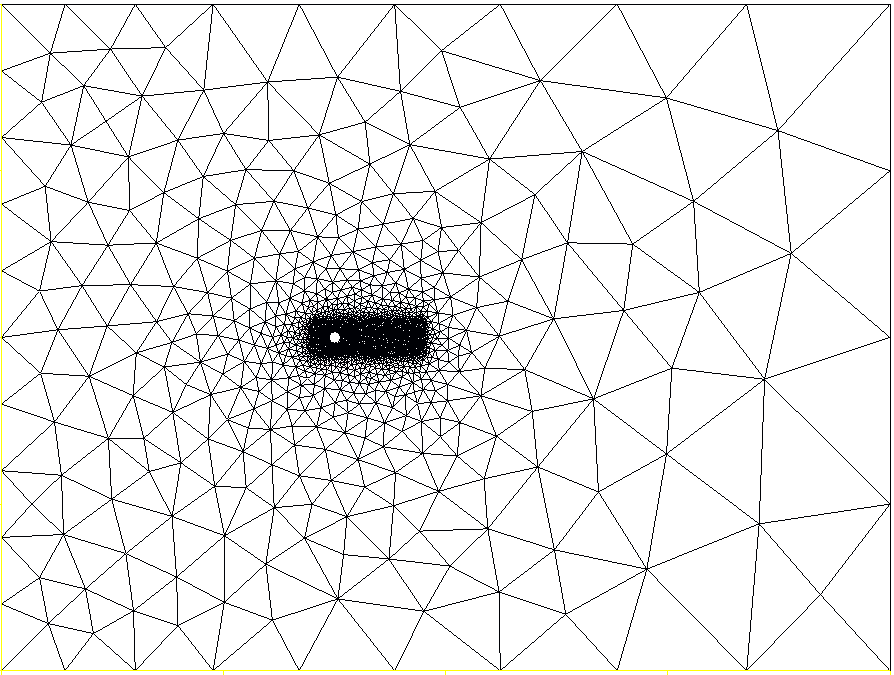
\includegraphics[width=0.55\textwidth]{\lfsdir/figs/cylinder_fine_v2.png}
}
\hfill
\subfloat[Close-up view \label{fig:mesh2_close}]{%
\centering
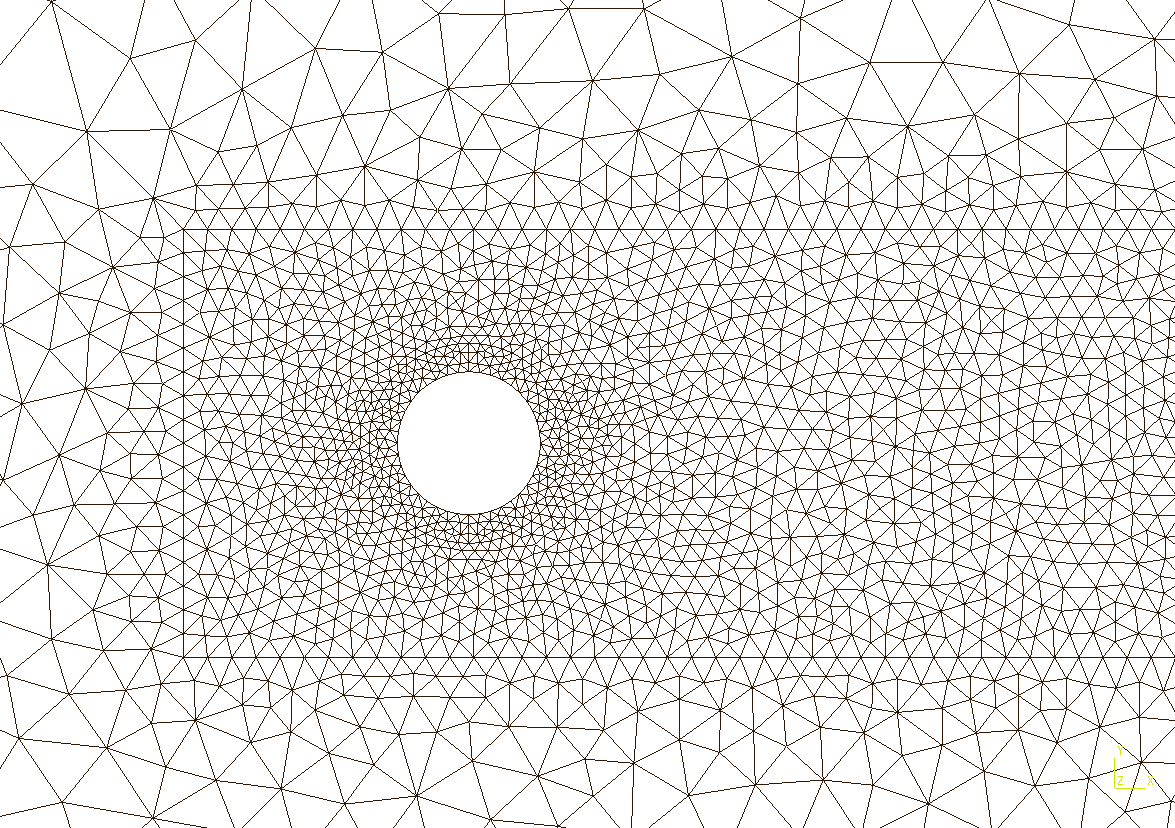
\includegraphics[width=0.55\textwidth]{\lfsdir/figs/mesh_closeup_2.png}
}
\caption{Unstructured, coarse mesh of a circular cylinder with 5,616 triangular elements. Elements adjacent to the cylinder have quadratic edges.}
\label{fig:meshes2}

\end{figure*}


\begin{figure*}
\hspace{-1cm}
\subfloat[Full view \label{fig:Ma0_0077Re1e6_Ma_far}]{%
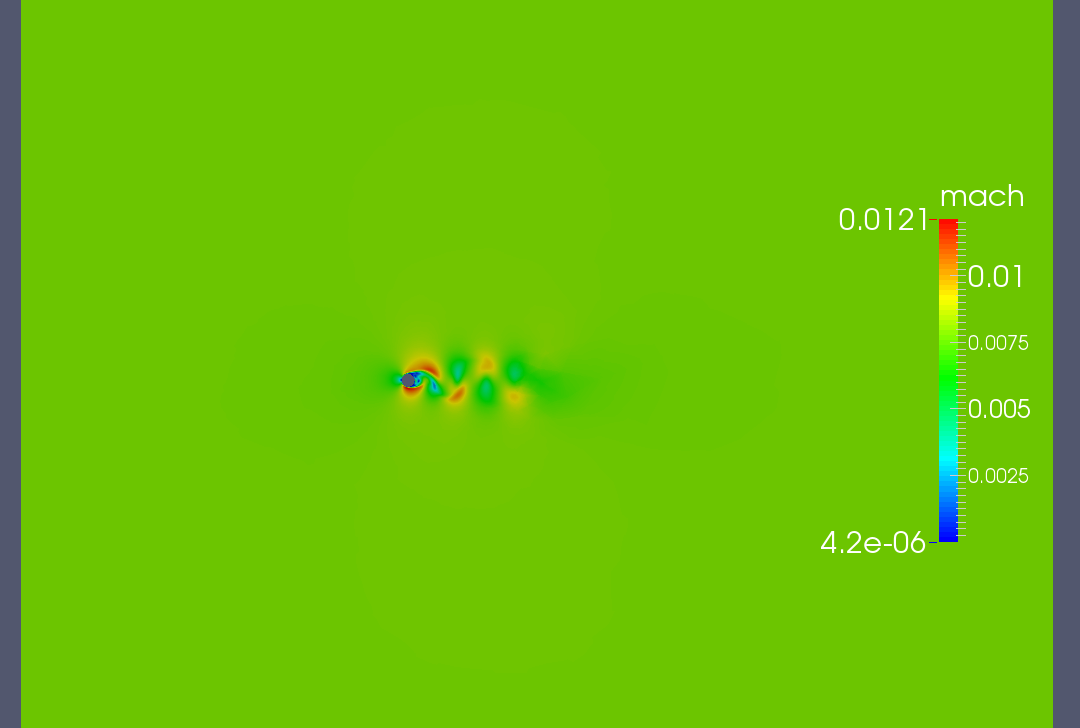
\includegraphics[width=0.55\textwidth]{\lfsdir/figs/Ma0_0077--Re1e6_Ma.png}
}
\hfill
\subfloat[Close-up view \label{fig:Ma0_0077Re1e6_Ma_close}]{%
\centering
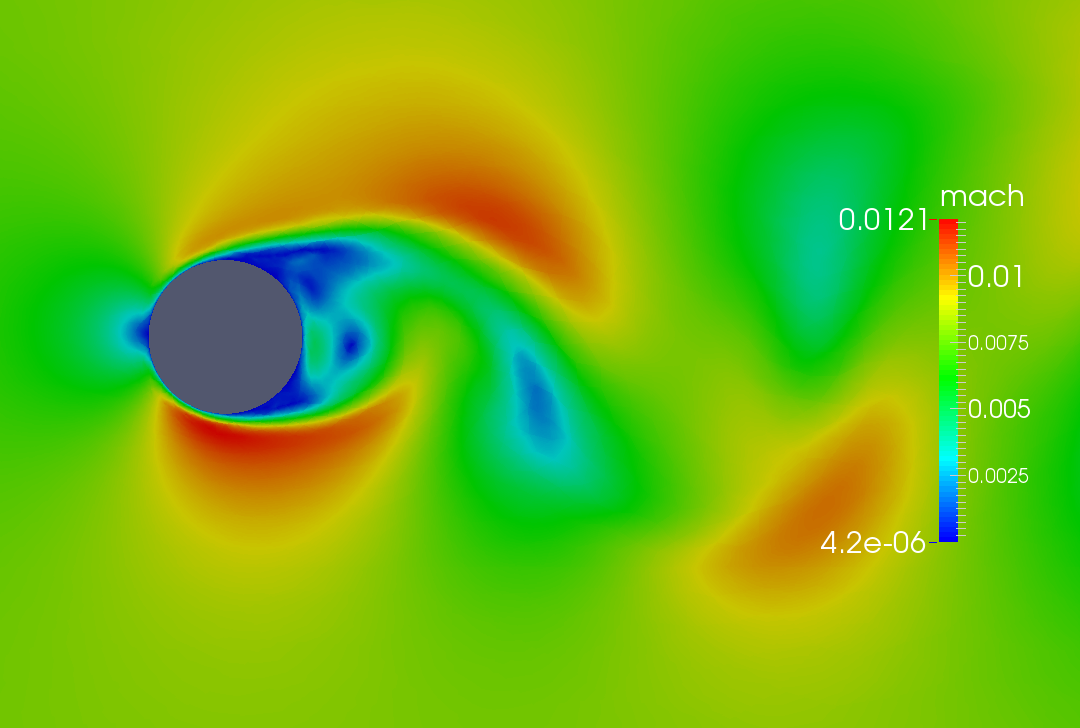
\includegraphics[width=0.55\textwidth]{\lfsdir/figs/Ma0_0077--Re1e6_Ma_closeup.png}
}
\caption{Flow past a cylinder. \gls{re}$= 1e6$, \gls{ma} $= 0.0077, p = 4$}
\label{fig:Ma0.0077Re1e6_Ma}

\end{figure*}



